\documentclass[12pt, a4paper, oneside]{article}
\usepackage{amsmath, amsthm, subcaption, float,amssymb, bm, graphicx, hyperref, mathrsfs, geometry}

\title{\large\textbf{STA2002 - Homework 2}}
\author{Xue Zhongkai 122090636}
\date{}
\linespread{1.5}
\geometry{a4paper, scale=0.8}
\newcounter{problemname}
\newenvironment{problem}{\stepcounter{problemname}\par\noindent\textsc{Problem \arabic{problemname}. }}{\\\par}

\begin{document}

\maketitle

% Problem 1
\begin{problem}
    \\
    (a)
    For point estimator $\hat{\mu_1}$, we have
    $$\mathbf{Bias} = \mathbb{E}(\frac{X_1}{3}+\frac{X_2}{3}+\frac{X_3}{3}) - \mu_1 = \frac{\mu_1}{3}+\frac{\mu_1}{3}+\frac{\mu_1}{3} - \mu_1 = 0$$
    For point estimator $\hat{\mu_2}$, we have
    $$\mathbf{Bias} = \mathbb{E}(\frac{X_1}{4}+\frac{X_2}{3}+\frac{X_3}{5}) - \mu_2 = \frac{\mu_2}{4}+\frac{\mu_2}{3}+\frac{\mu_2}{5} - \mu_2 = -\frac{13}{60}\mu_2$$
    As a result, $\hat{\mu_1}$ is unbiased.\\
    (b)
    For point estimator $\hat{\mu_1}$, we have
    $$\mathbf{Var}(\hat{\mu_1}) = \mathbf{Var}(\frac{X_1}{3}) + \mathbf{Var}(\frac{X_2}{3}) + \mathbf{Var}(\frac{X_3}{3}) = \frac{\mathbf{Var}(X_1)}{9} + \frac{\mathbf{Var}(X_2)}{9} + 
        \frac{\mathbf{Var}(X_3)}{9} = \frac{40}{9} \approx 4.444$$
    For point estimator $\hat{\mu_2}$, we have
    $$\mathbf{Var}(\hat{\mu_1}) = \mathbf{Var}(\frac{X_1}{4}) + \mathbf{Var}(\frac{X_2}{3}) + \mathbf{Var}(\frac{X_3}{5}) = \frac{\mathbf{Var}(X_1)}{16} + \frac{\mathbf{Var}(X_2)}{9} + 
    \frac{\mathbf{Var}(X_3)}{25} = \frac{1931}{720} \approx 2.682$$
    As a result, $\hat{\mu_2}$ has the smaller variance.\\
    (c)By equation $\mathbf{MSE} = \mathbf{Bias}^2 + \mathbf{Var}$, we have
    $$\mathbf{{MSE}_1} = \mathbf{{Bias}_1}^2 + \mathbf{{Var}_1} = 0 + \frac{40}{9} = \frac{40}{9} \approx 4.444$$
    $$\mathbf{{MSE}_2} = (\mathbf{{Bias}_2})^2 + \mathbf{{Var}_2} = -\frac{169}{3600}\mu_2 + \frac{1931}{720}  $$
    For $\mu =3$, we further have $$\mathbf{{MSE}_2} = \frac{2287}{900} \approx 2.541 < \mathbf{{MSE}_1}$$
    As a result, $\hat{\mu_2}$ has the smaller MSE.
\end{problem}

% Problem 2
\begin{problem}\\
    Assume all $X_i \geq \theta$, or the likelihood function is equal to 0 and it becomes trivial.\\
    $$\mathbf{L}(\theta) = f(x_1;\theta)f(x_2;\theta)\dots f(x_n;\theta) = \exp(n\theta - \sum_{i=1}^{n} x_i)$$
    Taking the logarithm, we have
    $$\mathbf{l}(\theta) = n \theta - \sum_{i=1}^{n} x_i  $$
    Taking the derivative, we have
    $$\frac{\partial}{\partial \theta} \mathbf{l}(\theta) = n > 0 \ ,$$
    which indicates $\mathbf{L}(\theta)$ is increasing mononiacally.\\
    To maximize $\mathbf{l}(\theta)$, $\theta$ should be as large as possible. \\
    As a result, $$\hat{\theta}_{mle} = \mathbf{min}(X_i) \ . $$
\end{problem}

% Problem 3
\begin{problem}
    \\
    (a)
    With the law of total probability, we have the joint probability
    $$ f(X, K) = f(X|K=0)P(k=0) + f(X|K=1)P(k=1)$$
    Since $X|K=0 \sim N(\mu_0, {\sigma_0}^2)$ and $X|K=1 \sim N(\mu_1, {\sigma_1}^2)$,
    \begin{equation*}
        f(X, K) =
        \left\{
            \begin{array}{lr}
                \frac{1}{\sigma_0 \sqrt{2\pi}}\exp[-\frac{(x-\mu_0)^2}{2\sigma_0^2}] \pi_0, & K_i = 0 \\
                \frac{1}{\sigma_1\sqrt{2\pi}}\exp[-\frac{(x-\mu_1)^2}{2\sigma_1^2}] \pi_1, & K_i = 1.\\     
            \end{array}
        \right.
    \end{equation*}
    \noindent
    (b)
    Denote the distribution of $(X, K)$ as $\mathbf{GMM}(\pi_0, \mu_0, \sigma_0^2, \mu_1, \sigma_1^2).$\\
    By $\mathbf{MLE}$, we can write the likelihood function as
    $$\mathbf{L}(\pi_0, \mu_0, {\sigma_0}^2, \mu_1, {\sigma_1}^2) 
    = \prod_{i=1}^{n}  \{ \frac{1}{\sigma_0 \sqrt{2\pi}}\exp[-\frac{(x-\mu_0)^2}{2\sigma_0^2}] \pi_0  \}^{1-K_i} 
                       \{ \frac{1}{\sigma_0 \sqrt{2\pi}}\exp[-\frac{(x-\mu_1)^2}{2\sigma_1^2}] \pi_1  \}^{K_i}
    $$
    Taking the logarithm,
    $$\mathbf{l} = \ln \mathbf{L} 
    = \sum_{i=1}^{n} (1-K_i) [\ln(\frac{\pi_0}{\sigma_0 \sqrt{2\pi}}) - \frac{(x-\mu_0)^2}{2\sigma_0^2}] + 
    \sum_{i=1}^{n} K_i [\ln(\frac{\pi_1}{\sigma_1 \sqrt{2\pi}}) - \frac{(x-\mu_1)^2}{2\sigma_1^2}] 
    $$
    Let $n_0$ and $n_1$ be the number of $X_i$ that belongs to group 0 and group 1 respectively.
    Taking the derivative $w.r.t$ each variable, 
    \begin{equation*}
        \left\{
            \begin{array}{lr}
                \frac{\partial}{\partial \pi_0} \mathbf{l} = \sum_{i=1}^{n} \frac{1-K_i}{\pi_0} + \sum_{i=1}^{n} \frac{K_i}{1-\pi_0} = \frac{n_0}{\pi_0} + \frac{n_1}{1-\pi_0} = 0\\
                \frac{\partial}{\partial \mu_0} \mathbf{l} = \sum_{i=1}^{n} (1-K_i)n_i - \mu_0 \sum_{i=1}^{n} (1-K_i) = 0\\
                \frac{\partial}{\partial \mu_1} \mathbf{l} = \sum_{i=1}^{n} K_i n_i - \mu_1 \sum_{i=1}^{n} K_i = 0\\
                \frac{\partial}{\partial \sigma_0^2} \mathbf{l} = -\sum_{i=1}^{n} \frac{1-K_i}{2\sigma_0^2} + \sum_{i=1}^{n} (1-K_i) \frac{(x_i - \mu_0)^2}{2 \sigma_0^2} = 0\\
                \frac{\partial}{\partial \sigma_1^2} \mathbf{l} = -\sum_{i=1}^{n} \frac{K_i}{2\sigma_1^2} + \sum_{i=1}^{n} (K_i) \frac{(x_i - \mu_1)^2}{2 \sigma_1^2} = 0\\
            \end{array}
        \right.
    \end{equation*}
    Solving the equation, we have
        $$\hat{\pi_0} = \frac{n_0}{n_0-n_1}, \ \
           \hat{\mu_0} = \frac{1}{n_0} \sum_{i=1}^{n}(1-K_i)x_i, \ \
           \hat{\mu_1} = \frac{1}{n_1} \sum_{i=1}^{n} K_i x_i 
        $$
        $$\hat{\sigma_0^2} = \frac{1}{n_0} \sum_{i=1}^{n} (1-K_i)(x_i-\hat{\mu_0})^2, \ \
           \hat{\sigma_1^2} = \frac{1}{n_1} \sum_{i=1}^{n} K_i (x_i-\hat{\mu_1})^2
        $$
\end{problem}

% Problem 4
\begin{problem}
    \\
    (a)
    Given $\sigma = 0.5$, $n = 20$, $1 - \alpha = 0.99$, two-sided estimation,
    $$\mathbf{z}_{\alpha/2} = \mathbf{z}_{0.005} = 2.5758, \ \ \
      \bar{x} = \frac{1}{11} \sum_{i = 1}^{11} = 13.755$$
    For lower bound of CI, $$\mu \geq \bar{x} - \mathbf{z}_{\alpha} \times \frac{\sigma}{\sqrt{n}}
                            = 13.755 - 2.5758 \times \frac{0.5}{\sqrt{20}} = 13.467$$
    For upper bound of CI, $$\mu \leq \bar{x} + \mathbf{z}_{\alpha} \times \frac{\sigma}{\sqrt{n}}
                            = 13.755 + 2.5758 \times \frac{0.5}{\sqrt{20}} = 14.043$$
    As a result, the confidence interval is $[13.467, 14.043].$  \\
    (b)
    Since $1 - \alpha = 0.95$, one-sided estimation,  
    $$\mathbf{z}_{\alpha} = \mathbf{z}_{0.05} = 1.6449$$
    For lower bound of CI, $$\mu \geq \bar{x} - \mathbf{z}_{\alpha} \times \frac{\sigma}{\sqrt{n}}
                            = 13.755 - 1.6449 \times \frac{0.5}{\sqrt{20}} = 13.571$$
    As a result, the confidence interval is $[13.571, + \infty).$\\
    (c)
    If $\bar{x}$ is used as an estimate of $\mu$, we can be 95\% (which implies, $\alpha = 0.05$) confident that the error $|\bar{x} - \mu|$
        will not exceed the specific amount $E$ when the sample size is 
        $$n = (\frac{\mathbf{z}_{\alpha/2}\sigma}{E})^2 = (\frac{1.96 \times 0.5}{2})^2 = 0.2401 \approx 1$$
    Therefore, a sample size of at least 1 would be required to achieve a 95\% CI.
\end{problem}

% Problem 5
\begin{problem}
    \\
    Since $n = 12$ and is sufficiently large, $\mathbf{CLT}$ could be applied.\\
    Using chi-square, we can estimate a CI for the variance $\sigma^2$
    $$\frac{(n-1)s^2}{\sigma^2} \sim \chi^2_{n-1}$$
    That is, $$P[\chi^2_{1-\alpha/2}(n-1) \leq \frac{(n-1)s^2}{\sigma^2} \leq \chi^2_{\alpha/2}(n-1)] = 1 - \alpha$$
    Construct a two-sided CI with $1-\alpha = 95\% $. That is,  $\alpha = 5\%$.\\
    For lower bound of CI, $$\sigma^2 \geq \frac{(n-1)s^2}{\chi^2_{\alpha/2}(n-1)} = \frac{(12-1)s^2}{\chi^2_{0.025}(12-1)} = \frac{11 \times 0.02445}{21.920} = 0.0123$$
    For upper bound of CI, $$\sigma^2 \geq \frac{(n-1)s^2}{\chi^2_{1-\alpha/2}(n-1)} = \frac{(12-1)s^2}{\chi^2_{0.975}(12-1)} = \frac{11 \times 0.02445}{3.816} = 0.0705$$
    As a result, the confidence interval is $[0.0123, 0.0705]$.
\end{problem}

% Problem 6
\begin{problem}
    According to the poll, the proportion of opposing is 32\%, and others is 68\%. \\
    For each of the individual as p = 32\%,
    $$X_i \sim Bernoulli(p)$$
    Since $n =1346$ and is sufficiently large, $\mathbf{CLT}$ could be applied as
    $$\hat{p} = \frac{\sum_{i=1}^{n} X_i}{n} \sim N(p, \frac{p(1-p)}{n})$$
    Build a two-sided CI with $1-\alpha = 95\%$, $\mathbf{z}_{\alpha/2} = \mathbf{z}_{0.025} = 1.96,$
    $$p \geq \hat{p} - \mathbf{z}_{\alpha/2}\sqrt{\frac{\hat{p}(1-\hat{p})}{n}} = 0.32 - 1.96\sqrt{\frac{0.32(1-0.32)}{1346}} \approx 0.295$$
    $$p \geq \hat{p} + \mathbf{z}_{\alpha/2}\sqrt{\frac{\hat{p}(1-\hat{p})}{n}} = 0.32 + 1.96\sqrt{\frac{0.32(1-0.32)}{1346}} \approx 0.345$$
    As a result, the confidence interval is $[0.295, 0.345].$  \\
    That is, we can be 95\% confident to confirm that the proportion of all American adults who oppose the legalization falls in the section of $[0.295, 0.345].$ 
\end{problem}

% Problem 7
\begin{problem}
    \\
    (a)(b)(c) The graph is as follows:
    \begin{figure}[H]
    \begin{subfigure}{0.4\textwidth}
        \centering
        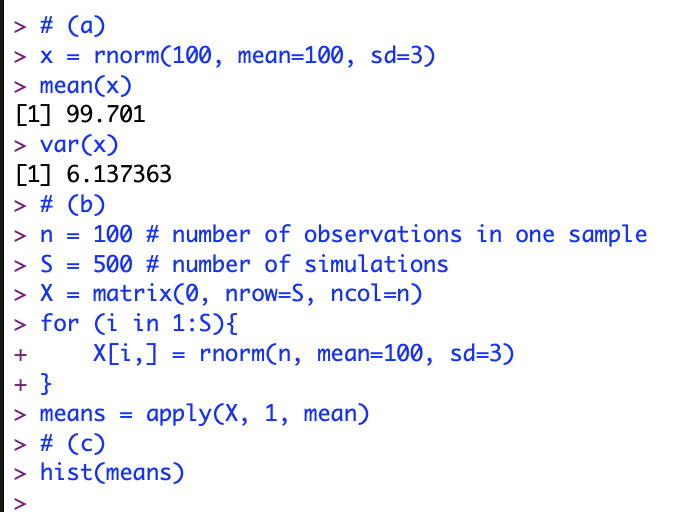
\includegraphics[width=\linewidth]{code-1.png}
        \caption{Code}
        \label{fig:sub1}
    \end{subfigure}
    \hfill
    \begin{subfigure}{0.4\textwidth}
        \centering
        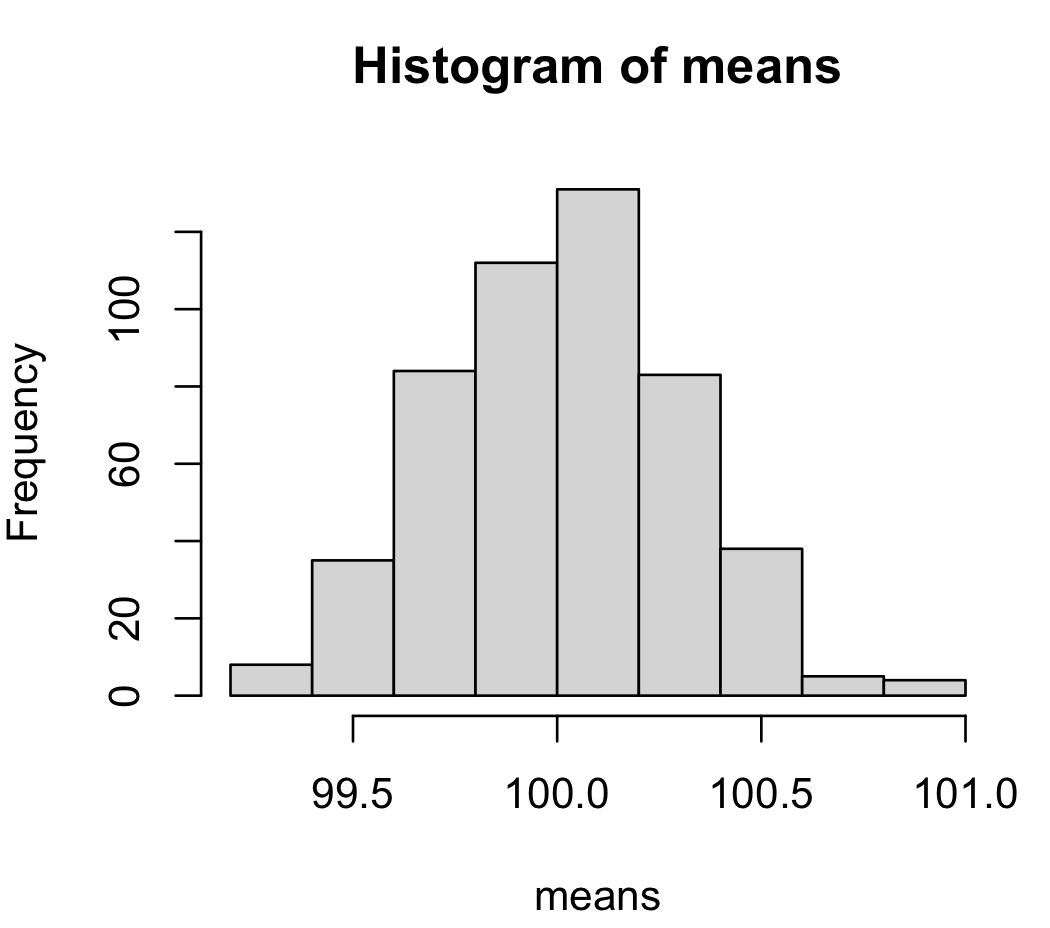
\includegraphics[width=\linewidth]{plot-1.png}
        \caption{Plot}
        \label{fig:sub2}
    \end{subfigure}
    \end{figure}
   \noindent 
   (d)For the theoretical sampling distribution with $s^2 = \frac{\sigma^2}{500} = 0.018$,
    $$\hat{\mu} \sim N(100, 0.018)$$
    The hisgram seems quite normal, with a standard symmetry bell-characteristic. \\
    As a result, the hisgram could approximate the sampling well.
\end{problem}


\end{document}